\chapter{Asset Class Returns modeling}\label{chpt:assetclass_returns}
	
In this chapter, we address the asset class returns modeling issue. As it was noted above, the ODAA algorithm does not depend on a particular distribution for the asset class returns vector $\bm{w}_{k+1}$. However, by looking at equation  (\ref{eq:rec_algo}) we see that we need the explicit analytical form for the density function $p_{f(x,\bm{u}_k,\bm{w}_{k+1})}$. For this reason, we will be dealing exclusively with probability distributions closed under linear combination. In this work, we propose three such distributions:
\begin{itemize}
	\item Gaussian
	\item Gaussian Mixture
	\item Generelized Hyperbolic
\end{itemize}
For each of them, first we will give a theoretical introduction, secondly derive the portfolio value density function $p_{f(x,\bm{u}_k,\bm{w}_{k+1})}$ and an expression for the risk constraint (which depends on the distribution chosen).
\section{Gaussian model}
The first probability distribution we considered is the Gaussian 
\begin{definition}[Gaussian random vector]\label{def:gauss_rv}
	A $m$-dimensional random vector $\bm{w} = [w_1,\ldots,w_m]^T$ is \textbf{Gaussian} if every linear combination $\sum_{i=0}^{m}u_iw_i = \bm{u}^T \bm{w}$ has a one-dimensional Gaussian distribution.
\end{definition}
Let the asset class returns random vector $\bm{w}_{k+1}$ follow a Gaussian distribution with mean $\bm{\mu}$ and covariance matrix $\bm{\Sigma}$  $\big(\bm{w}_{k+1} \sim \mathcal{N}(\bm{\mu},\bm{\Sigma})\big)$. By definition we have \[x(1 + \bm{u}_k^T \bm{w}_{k+1}) \sim \mathcal{N}\Big(\underbrace{x(1 + \bm{u}_k^T \bm{\mu})}_{\tilde{\mu}}, \underbrace{x^2\bm{u}_k^T \Sigma \bm{u}_k}_{\tilde{\sigma}^2}\Big)\]
hence
\begin{equation}
\boxed{p_{f(x,\bm{u}_k,\bm{w}_{k+1})}(z) =  \frac{1}{\sqrt{2\pi}\tilde{\sigma}}\exp\big\{ -\frac{1}{2}\frac{(z-\tilde{\mu})^2}{\tilde{\sigma}^2}\big\}, \quad z \in \mathbb{R}.}
\end{equation}
 

Let us now introduce the two important concepts of loss function and value-at-risk that we will use to derive the portfolio risk constraint
\begin{definition}[loss function]\label{def:loss_function}
	Denoting the value of our portfolio at time $k \in \mathbb{N}$ by $x_{k+1}$, the \textbf{loss function} of the portfolio over the period $[k,k+1]$ is given by \[ L_{k+1}:= -\frac{(x_{k+1}-x_k)}{x_k}= -r_{k+1} = -\bm{u}_k^T \bm{w}_{k+1}.  \]
\end{definition}
\begin{definition}[Value-at-risk]
	Given some confidence level $1-\alpha \in (0,1) $ the \textbf{value-at-risk} ($V@R_{1-\alpha}$) of our portfolio is \[ V@R_{1-\alpha} = \inf\{l\in \mathbb{R} : \mathbb{P}\big(L_{k+1} \leq l \big) \geq 1-\alpha \}. \]
\end{definition}
	

The V@R is a risk measure commonly use by financial institutions to asses the risk they run to carry a portfolio for a specified period of time (the portfolio must be kept constant during this time period). For instance, if our portfolio has a $V@R_{0.99} = 7\%$, this means that with a confidence level of $99\%$ our portfolio does not suffer a loss greater or equal than $7\%$ over per period $[k,k+1]$ (e.g. a month). In our case, we receive the V@R specification ($V@R_{0.99} = 7\%$) in input by the investor (it is an indicator of its risk-aversion) and we will construct an asset allocation $\bm{u}_k$ that satisfies this risk constraint at each $k \in \mathbb{N}$.

Using definition (\ref{def:gauss_rv}) we have \[ L_{k+1} \sim \mathcal{N}\big(\underbrace{-\bm{u}_k^T \bm{\mu}}_{\mu_p},\underbrace{\bm{u}_k^T \bm{\Sigma} \bm{u}_k}_{\sigma^2_p} \big)\] therefore
\begin{align*}
\mathbb{P}\big(L_{k+1} \leq V@R_{1-\alpha}\big) 
& = \mathbb{P}\Big(Z \leq \frac{V@R_{1-\alpha} - \mu_p}{\sigma_p}  \Big) \\
& = 1 - \alpha
\end{align*}
\begin{equation}\label{eq:var_const_gaussian}
\implies \boxed{V@R_{1-\alpha} \geq -\bm{u}_k^T\bm{\mu} + z_{1-\alpha} \sqrt{\bm{u}_k^T \bm{\Sigma} \bm{u}_k}}
\end{equation}
where $Z$ is a standard normal random variable and $z_{1-\alpha}$ is the $1-\alpha$ quantile of the standard normal distribution. The \textit{risk} constraint in equation (\ref{eq:var_const_gaussian}), together with the \textit{budget} and \textit{long-only} constraint, define the control space $U_k$ which is the feasible set of the constrained optimization problem given in theorem (\ref{thm:rec_algo}).
\section{Gaussian Mixture model}
In this section we present the second asset class returns model, the \textbf{Gaussian Mixture model} (GM). After introducing the GM distribution we will derive the density and the \textit{risk} constraint, as we did for the Gaussian model. We closely follow \cite{BUCKLEY2008}.

The standard assumption that asset returns have a multivariate Gaussian distribution is a reasonable first approximation to reality and it usually has the big advantage of generating analytically tractable theories (e.g. Markowitz portfolio theory). However, the Gaussian model does not capture two important key features of asset returns which are observed in the market real data:
\begin{enumerate}
	\item the skewed (asymmetric around the mean) and leptokurtic (more fat-tailed than the Gaussian) nature of marginal probability density function
	\item the asymmetric correlation between asset returns, that is the tendency of volatilities and correlations to depend on the prevailing market conditions.
\end{enumerate}
To overcome this shortcomings, the Gaussian Mixture distribution is a validate alternative to the Gaussian one. Loosely speaking, the pdf of a GM random vector id a linear combination of Gaussian pdfs (called Gaussian regimes or mixing components). This closeness to the Normal distribution offers a good trade-off between analytical tractability and parsimony in the number of parameters. By adopting a GM model, it is possible to represent protuberances on the probability iso-density contour, as can be seen in the following figure
\begin{figure}[H]
	\caption{Example of a GM density contour plot with two mixing components.}
	\centering
	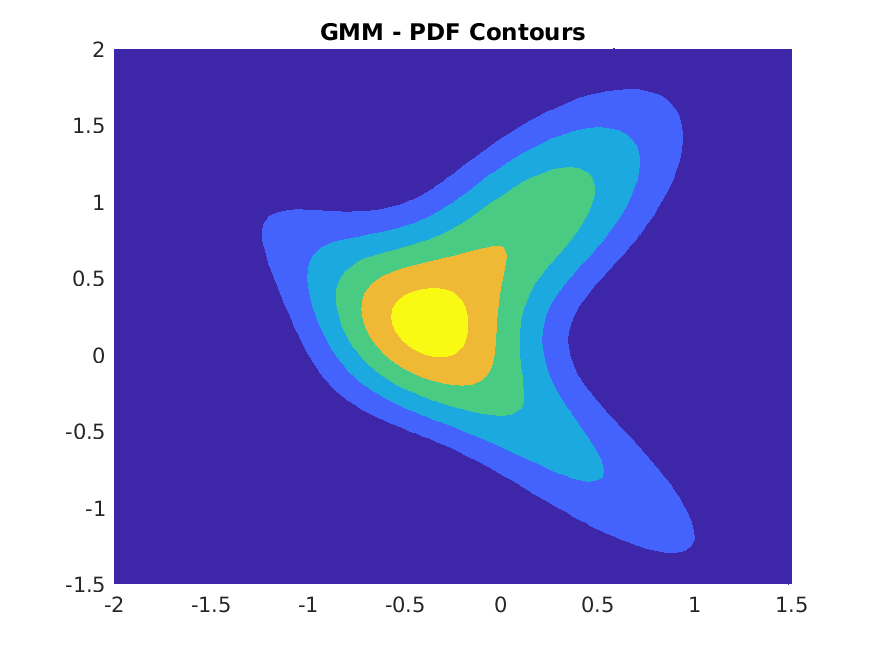
\includegraphics[width=0.7\textwidth]{Images/GMdensity.png}
\end{figure}
To obtain this highly non-linear dependence structure, we would usually need cross-moments of all order; a big advantage of the GM distribution is that its dependence structure is fully and conveniently captured by the means, covariance matrices and weights of each Gaussian regime (as we will see in the following).

We start the more formal introduction on the GM distribution giving its definition
\begin{definition}[GM distribution]
	An $m$-dimensional random vector $\bm{Z}$ has a \textbf{multivariate GM distribution} if its probability density function is of the form
	\[ p_{\bm{Z}}(\bm{z}) = \sum_{i=1}^{n} \lambda_i \varphi_{(\bm{\mu}_i,\bm{\Sigma}_i)}(\bm{z}), \quad \bm{z} \in \mathbb{R}^m, \] 
	where $\varphi_{(\bm{\mu}_i,\bm{\Sigma}_i)}$ is the multivariate Gaussian density with mean vector $\bm{\mu}_i$ and covariance matrix $\bm{\Sigma}_i$ and $\lambda_i$ are positive mixing weights summing to one.	
\end{definition}
The following proposition is crucial for our purposes since it tells us that linear combinations of GM random vector have a one-dimensional GM distribution
\begin{proposition}\label{prop:GM_lin_comb}
	Linear combinations of GM random vectors follow a univariate GM distribution. In particular, if $\bm{Z} \sim GM$ then $Y=\bm{\theta}^T \bm{Z}$,  $\forall \bm{\theta} \in \mathbb{R}^m$, has a GM distribution with probability density function \[ p_Y(y) = \sum_{i=1}^{n}\lambda_i \varphi_{(\mu_i,\sigma_i^2)}(y),\quad y \in \mathbb{R} \] where
	\[
	\begin{cases}
	\mu_i & = \bm{\theta}^T \bm{\mu}_i \quad i = 1,\ldots,m \\
	\sigma_i^2 & = \bm{\theta}^T \bm{\Sigma}_i \bm{\theta} \quad i = 1,\ldots,m
	\end{cases} \]
\end{proposition}
\begin{proof}
	The characteristic function (CF) of a GM random vector is the linear combination of the CF of the Gaussian mixing components. Indeed 
	\begin{align*}
	\phi_{\bm{Z}}(\bm{u}) &= \mathbb{E}[\exp\{i \bm{u}^T \bm{Z}\} ] = \int_{\mathbb{R}^m}\exp\{i \bm{u}^T \bm{z}\}p_{\bm{Z}}(\bm{z})\mathrm{d}\bm{z} = \\
	& = \int_{\mathbb{R}^m}\exp\{i \bm{u}^T \bm{z}\}\sum_{i=1}^{n}\lambda_i \varphi_{(\bm{\mu}_i,\bm{\Sigma}_i)}(\bm{z})\mathrm{d}\bm{z} = \\
	& = \sum_{i=1}^{n}\lambda_i \phi_{\bm{X}_i}(\bm{u}), \quad \bm{u} \in \mathbb{R}^m
	\end{align*}
	where $\bm{X}_i \sim \mathcal{N}\big(\bm{\mu}_i,\bm{\Sigma}_i\big)$. Therefore, $\forall \bm{\theta} \in \mathbb{R}^m$ we have
	\begin{align*}
	\phi_{\bm{\theta}^T \bm{Z}}(u) & = \mathbb{E}[\exp\{iu(\bm{\theta}^T\bm{Z})\}] = \mathbb{E}[\exp\{i(u\bm{\theta}^T)\bm{Z}\}] = 
    \phi_{\bm{Z}}(u\bm{\theta}) = \\
    & = \sum_{i=1}^{n}\lambda_i \phi_{X_i}(u\bm{\theta}) = \sum_{i=1}^{n}\lambda_i \exp\{iu\underbrace{\bm{\theta}^T\bm{\mu}_i}_{\mu_i}-\frac{1}{2}u^2\underbrace{\bm{\theta}^T\bm{\Sigma}_i\bm{\theta}}_{\sigma_i^2}\} = \\
	& = \sum_{i=1}^{n}\lambda_i \phi_{\widetilde{X}_i}(u), \quad u \in \mathbb{R}
	\end{align*}
	where $\widetilde{X}_i \sim \mathcal{N}\big(\mu_i,\sigma_i^2 \big)$. Since the CF completely characterizes the distribution (see theorem 14.1 in \cite{jacod2000probability}) we have the result.
\end{proof}
Suppose the asset class returns vector\footnote{for the sake of clarity we drop the subscript $k+1$ when it is not needed} $\bm{w}$ follow a Gaussian Mixture distribution ($\bm{w} \sim GM $). We want to compute the density of random variable $f(x,\bm{u},\bm{w}) = x(1 + \bm{u}^T\bm{w})$. Thanks to proposition (\ref{prop:GM_lin_comb}) we know that the random variable $\bm{u}^T\bm{w}$ follows itself a GM (univariate) distribution. Moreover, by integration we easily derive its cumulative distribution function (CDF) allowing us to write
\begin{align*}
F_{f(x,\bm{u},\bm{w})}(z) & = \mathbb{P}\big(x(1+\bm{u}^T\bm{w})\leq z \big) = F_{x\bm{u}^T\bm{w}}(z-x)\\
& = \sum_{i=1}^{n}\lambda_i \Phi\Big(\frac{z - x(1+\bm{u}^T\bm{\mu}_i)}{\sqrt{x^2\bm{u}^T\bm{\Sigma}_i\bm{u}}}\Big), \quad z \in \mathbb{R}
\end{align*}
where $\Phi$ is the standard normal CDF. Differentiating with respect to $z$, we have
\begin{equation}
\boxed{p_{f(x,\bm{u},\bm{w})}(z) = \sum_{i=1}^{n}\lambda_i \varphi_{(\mu_i,\sigma_i^2)}(z), \quad z \in \mathbb{R}}
\end{equation}
where 
\[
\begin{cases}
	\mu_i &= x(1+\bm{u}^T \bm{\mu}_i) \\
	\sigma_i^2 & = x^2\bm{u}^T\bm{\Sigma}_i \bm{u}.
\end{cases}
\]


We now turn to the problem of computing the \textit{risk} constraint under the GM distribution assumption. We will follow two different approaches. Suppose we are given the $V@R_{1-\alpha}$ specification (e.g. $7\%$); by using definition (\ref{def:loss_function}) we have \[ \mathbb{P}\big(L \leq V@R_{1-\alpha} \big) = F_L(V@R_{1-\alpha}) \geq 1-\alpha \] as noted above, the CDF of $L = -\bm{u}^T \bm{w}$ is known, therefore \[\sum_{i=1}^{n}\lambda_i \Phi\Big(\frac{V@R_{1-\alpha} - \mu_i}{\sigma_i}\Big) \geq 1-\alpha \quad \implies \quad\]
\begin{equation}
 \boxed{\sum_{i=1}^{n}\lambda_i \Phi\Big(-\Big\{\frac{V@R_{1-\alpha} - \mu_i}{\sigma_i} \Big\} \Big) \leq \alpha}  
\end{equation}
where \[
\begin{cases}
\mu_i & = -\bm{u}^T \bm{\mu}_i \\
\sigma_i^2 & = \bm{u}^T \bm{\Sigma}_i \bm{u}.
\end{cases}\]
We present also an alternative method to limit the risk exposure of our portfolio which turns out to be less computationally intensive. The idea is to set an upper bound to portfolio return volatility in the following way 
\begin{equation}\label{eq:risk_upperbnd}
(\Var{r_{k+1}})^{\frac{1}{2}} = (\bm{u}_k^T \bm{\Lambda} \bm{u}_k)^{\frac{1}{2}} \leq \sigma_{max}
\end{equation}
where $\bm{\Lambda}$ is the covariance matrix of vector $\bm{w}_{k+1}$. Two questions are left open: how to compute $\bm{\Lambda}$ and how to link the upper bound $\sigma_{max}$ to the $V@R_{1-\alpha}$ specification given in input by the investor. As far as the former is concerned, the following proposition gives us the answer
\begin{proposition}
	The covariance matrix of a random vector with the GM distribution can be expressed in terms of mean vectors, covariance matrices and weights of the mixing components in the following way
	\[ \bm{\Lambda} = \sum_{i=1}^{n}\lambda_i\bm{\Sigma}_i + \sum_{i=1,j<i}^{n,n} \lambda_i\lambda_j(\bm{\mu}_i-\bm{\mu}_j)(\bm{\mu}_i-\bm{\mu}_j)^T.\]
\end{proposition}
To answer the latter, we use a Guassian approximation and the fact that if the rebalancing frequency is relatively small (e.g. weekly) the portfolio return mean is negligible. In the end, the obtain
\[ \sigma_{max} = \frac{V@R_{1-\alpha}}{z_{1-\alpha}}. \] 
\section{Generelized Hyperbolic model}
The last distribution we propose for our asset class returns modeling purposes is the Generalized Hyperbolic (GH). Like the GM, in its general form also the GH presents a non-elliptical behaviour with asymmetric and fat-tailed marginals. We proceed to give the formal definition and then derive the density of $f(x,\bm{u}_k,\bm{w}_{k+1})$
and the \textit{risk} constraint.
\begin{definition}[GH distribution]\label{def:GH}
	A $m$-dimensional random vector $\bm{X}$ is said to follow a \textbf{multivariate GH distribution} ($\bm{X} \sim GM_m(\lambda,\chi,\psi,\bm{\mu},\bm{\Sigma},\bm{\gamma})$) if \[ \bm{X} = \bm{\mu}+W\bm{\gamma}+\sqrt{W}A\bm{Z} \] where 
	\begin{itemize}
		\item $\bm{Z} \sim \mathcal{N}\big(\bm{0},I_d\big)$
		\item $A \in \mathbb{R}^{m \times d} $ is the Cholesky factor of dispersion matrix $\bm{\Sigma}$ ($A^TA = \bm{\Sigma}$)
		\item $\bm{\mu}, \bm{\gamma} \in \mathbb{R}^m$
		\item $W \sim \mathcal{N}^-(\lambda,\chi,\psi)$, $W \geq 0$ and $W \perp \bm{Z}$ (see Appendix \ref{app:B} for the definition of the GIG distribution). $W$ is sometimes called mixing random variable.
	\end{itemize}
\end{definition}
\begin{remark}
	\begin{itemize}
		\item $\lambda,\chi,\psi$ are shape parameters; the larger these parameters the closer the distribution is to the Gaussian
		\item $\bm{\gamma}$ is the skewness parameter. If $\bm{\gamma}= \bm{0}$ the distribution is symmetric around the mean
		\item $\bm{X}\lvert W = w \sim \mathcal{N}\big(\bm{\mu}+w\bm{\gamma},w\bm{\Sigma}\big)$
	\end{itemize}
\end{remark}
The GH distribution contains some special cases:
\begin{itemize}
	\item If $\lambda=\frac{m+1}{2}$ we have a \textit{Hyperbolic} distribution
	\item If $\lambda=-\frac{1}{2}$ the distribution is called \textit{Normal Inverse Gaussian} (NIG)
	\item If $\chi = 0$ and $\lambda > 0$ we have the limiting case of the \textit{Variance Gamma} (VG) distribution
	\item If $\psi = 0$ and $\lambda < 0$ the resulting distribution is called \textit{Student-t}.
\end{itemize}
	
The following proposition gives us the closeness under linear transformation that we need for our modeling purposes
\begin{proposition}
	If $\bm{X} \sim GH_m(\lambda,\chi,\psi,\bm{\mu},\bm{\Sigma},\bm{\gamma})$ and $\bm{Y}=B\bm{X}+\bm{b}$, where $B \in \mathbb{R}^{d\times m}$ and $\bm{b} \in \mathbb{R}^d$, then
	\[ \bm{Y} \sim GH_d(\lambda,\chi,\psi,B\bm{\mu}+b,B\bm{\Sigma}B^T,B\bm{\gamma}). \]
\end{proposition}
Suppose $\bm{w}_{k+1} \sim GH_m(\lambda,\chi,\psi,\bm{\mu},\bm{\Sigma},\bm{\gamma})$. Applying the previous result to our case $\big(Y = f(x,\bm{u}_k, \bm{w}_{k+1}),\quad B=x\bm{u}_k^T,\quad b = x\big)$ we have \[ f(x,\bm{u}_k,\bm{w}_{k+1}) \sim GH_1(\lambda,\chi,\psi,\underbrace{x(1+\bm{u}_k^T\bm{\mu})}_{\widetilde{\mu}},\underbrace{x^2\bm{u}_k^T\bm{\Sigma}\bm{u}_k}_{\widetilde{\Sigma}},\underbrace{x\bm{u}_k^T\bm{\gamma}}_{\widetilde{\gamma}}) \] and the density reads as (see Appendix  \ref{app:B})
\begin{equation}\label{eq:GHdensity}
\boxed{p_{f(x,\bm{u}_k, \bm{w}_{k+1})}(z) = c \frac{K_{\lambda-\frac{1}{2}}\Big(\sqrt{\big(\chi+\widetilde{Q}(z) \big)\big(\psi+\widetilde{\gamma}^2/\widetilde{\Sigma} \big)\exp\big\{(z-\widetilde{\mu})\widetilde{\gamma}/\widetilde{\Sigma} \big\}}\Big)}{\Big(\sqrt{\big(\chi+\widetilde{Q}(z) \big)\big(\psi+\widetilde{\gamma}^2/\widetilde{\Sigma} \big)}\Big)^{\frac{1}{2}-\lambda}}}
\end{equation}
where \[ c = \frac{\big(\sqrt{\chi\psi}\big)^{-\lambda}\psi^{\lambda}\big(\psi+\widetilde{\gamma}^2/\widetilde{\Sigma}\big)^{\frac{1}{2}-\lambda}}{(2\pi\widetilde{\Sigma})^{\frac{1}{2}}K_{\lambda}(\sqrt{\chi\psi})} \]
and $\widetilde{Q}(z)= (z-\widetilde{\mu})/\widetilde{\Sigma}$.


As far as the \textit{risk} constraint is concerned, we adopt here the alternative approach expressed in Equation (\ref{eq:risk_upperbnd}). The covariance matrix $\bm{\Lambda}$ is easily derived from the definition of a GH random vector (Definition (\ref{def:GH})) and Equation (\ref{eq:GIG_moment}) in Appendix \ref{app:B}; in the end we obtain
\begin{equation}
\bm{\Lambda} = \Var{W}\bm{\gamma}\bm{\gamma}^T+\mathbb{E}[W]\bm{\Sigma}
\end{equation}
where
\begin{align*}
\mathbb{E}[W] & = \Big(\frac{\chi}{\psi}\Big)^{\frac{1}{2}}\frac{K_{\lambda+1}(\sqrt{\chi\psi})}{K_{\lambda}(\sqrt{\chi\psi})}\\
\Var{W} & = \Big(\frac{\chi}{\psi}\Big)\frac{1}{K_{\lambda}(\sqrt{\chi\psi})}\Big\{K_{\lambda+2}(\sqrt{\chi\psi})-\frac{K_{\lambda+1}^2(\sqrt{\chi\psi})}{K_{\lambda}(\sqrt{\chi\psi})} \Big\}.
\end{align*}



